%%%%%%%%%%%%%%%%%%%%%%%%%%%%%%%%%%%%%%%%%%%%%%%%%%%%%%%%%%%%%%%%%%%%%%
%%%%%%%%%%%%%%%%%%%%%%%%%%%%%%%%%%%%%%%%%%%%%%%%%%%%%%%%%%%%%%%%%%%%%%
%%%%% Configuration %%%%%%%%%%%%%%%%%%%%%%%%%%%%%%%%%%%%%%%%%%%%%%%%%%
%%%%%%%%%%%%%%%%%%%%%%%%%%%%%%%%%%%%%%%%%%%%%%%%%%%%%%%%%%%%%%%%%%%%%%
%%%%%%%%%%%%%%%%%%%%%%%%%%%%%%%%%%%%%%%%%%%%%%%%%%%%%%%%%%%%%%%%%%%%%%

\documentclass[
	a4paper,	% feuille A4
	twoside,	% impression Recto-Verso
	12 pt		% taille de police
]{report}		% type de document


%%%%%%%%%% Extensions %%%%%%%%%%
\usepackage[utf8]{inputenc}		% encodage des caractères
\usepackage[T1]{fontenc}		% nouvelle norme de codage
\usepackage[francais]{babel}	% langue française
\usepackage{multicol}			% multi-colonnes
\usepackage{graphicx}			% images


%%%%%%%%%% Marges %%%%%%%%%%
\usepackage[
	tmargin = 2.5 cm,	% haut
	bmargin = 5 cm,		% bas
	lmargin = 2.5 cm,	% gauche
	rmargin = 2.5 cm	% droite
]{geometry}


%%%%%%%%%% Inter-ligne %%%%%%%%%%
\usepackage{setspace}
\onehalfspacing			% 1.5


%%%%%%%%%% Code source %%%%%%%%%%
\usepackage{listings}
\lstset{
	aboveskip = -1 pt,			% espace au dessus de la zone
	basicstyle = \ttfamily,		% caractères de même taille
	belowskip = -1 pt,			% espace en dessous de la zone
	showstringspaces = false,	% masquer les espaces
	tabsize = 4,				% nombre d'espace par tabulation
	xleftmargin = 30 pt,		% marge à gauche
	xrightmargin = 0 pt,		% marge à droite
}


%%%%%%%%%% Informations %%%%%%%%%%
\title{Développement d'une application de recrutement}
\author{\href{mailto:pinguet62@gmail.com}{Julien PINGUET}}
\date{Avril-Septembre 2013}


%%%%%%%%%% Liens %%%%%%%%%%
\usepackage{hyperref}
\hypersetup{ 			% Options : http://forum.ubuntu-fr.org/viewtopic.php?id=81505%29
	backref = true,
	pagebackref = true,	% dans bibliographie
	pdfborder = {0 0 0}	% retirer le cadre
}


%%%%%%%%%% Glossaire %%%%%%%%%%
%\usepackage{glossaries}
%\makeglossaries
%\cleardoublepage

\chapter*{Glossaire}

\addcontentsline{toc}{chapter}{Glossaire}
\markboth{Glossaire}{}



TODO: commandes LaTeX

Bibliothèque : TODO

Framework : ensemble de composants logiciels permettant le développement le développement rapide d'applications.


%%%%%%%%%% En-tête et Pied de page %%%%%%%%%%
\usepackage{fancyhdr}
\pagestyle{fancyplain}

\makeatletter % début d'utilisation des variables @



%%%%%%%%%%%%%%%%%%%%%%%%%%%%%%%%%%%%%%%%%%%%%%%%%%%%%%%%%%%%%%%%%%%%%%%%%%%%%%%%%%%%%%%%%%%%%%%%%%%%
%%%%% Page vides %%%%%%%%%%%%%%%%%%%%%%%%%%%%%%%%%%%%%%%%%%%%%%%%%%%%%%%%%%%%%%%%%%%%%%%%%%%%%%%%%%%
%%%%%%%%%%%%%%%%%%%%%%%%%%%%%%%%%%%%%%%%%%%%%%%%%%%%%%%%%%%%%%%%%%%%%%%%%%%%%%%%%%%%%%%%%%%%%%%%%%%%

\fancypagestyle{empty}{
	% Effacer les valeurs par défaut
	\fancyhf{}
	
	% Remplissage
	\lhead	[]								% haut	gauche	pair
			{}								% haut	gauche	impair
	\chead	[]								% haut	centre	pair
			{}								% haut	centre	impair
	\rhead	[]								% haut	droite	pair
			{}								% haut	droite	impair
	\lfoot	[]								% bas	gauche	pair
			{}								% bas	gauche	impair
	\cfoot	[]								% bas	centre	pair
			{}								% bas	centre	impair
	\rfoot	[]								% bas	droite	pair
			{}								% bas	droite	impair
	
	% Epaisseur de la ligne séparatrice
	\renewcommand{\headrulewidth}{0 pt}		% en-tête (défaut : 0.4pt)
	\renewcommand{\footrulewidth}{0 pt}		% pied de page (défaut : 0pt)
	
	% Distance du corps
	\headsep = 25 pt						% en-tête (défaut : 25pt)
	\footskip = 75 pt						% pied de page (défaut : 30pt)
}



%%%%%%%%%%%%%%%%%%%%%%%%%%%%%%%%%%%%%%%%%%%%%%%%%%%%%%%%%%%%%%%%%%%%%%%%%%%%%%%%%%%%%%%%%%%%%%%%%%%%
%%%%% Page des chapitre (défaut) %%%%%%%%%%%%%%%%%%%%%%%%%%%%%%%%%%%%%%%%%%%%%%%%%%%%%%%%%%%%%%%%%%
%%%%%%%%%%%%%%%%%%%%%%%%%%%%%%%%%%%%%%%%%%%%%%%%%%%%%%%%%%%%%%%%%%%%%%%%%%%%%%%%%%%%%%%%%%%%%%%%%%%%

\fancypagestyle{plain}{
	% Effacer les valeurs par défaut
	\fancyhf{}
	
	% Remplissage
	\lhead	[\large \bf \fbox{\thepage}]	% haut	gauche	pair	:	numéro de page
			{}								% haut	gauche	impair
	\chead	[]								% haut	centre	pair
			{}								% haut	centre	impair
	\rhead	[]								% haut	droite	pair
			{\large \bf \fbox{\thepage}}	% haut	droite	impair	:	numéro de page
	\lfoot	[\@title]						% bas	gauche	pair	:	titre du rapport
			{\@author}						% bas	gauche	impair	:	auteur du rapport
	\cfoot	[]								% bas	centre	pair
			{}								% bas	centre	impair
	\rfoot	[\@author]						% bas	droite	pair	:	auteur du rapport
			{\@title}						% bas	droite	impair	:	titre du rapport
	
	% Epaisseur de la ligne séparatrice
	\renewcommand{\headrulewidth}{0 pt}		% en-tête (défaut : 0.4pt)
	\renewcommand{\footrulewidth}{0.4 pt}	% pied de page (défaut : 0pt)
	
	% Distance du corps
	\headsep = 25 pt						% en-tête (défaut : 25pt)
	\footskip = 75 pt						% pied de page (défaut : 30pt)
}



%%%%%%%%%%%%%%%%%%%%%%%%%%%%%%%%%%%%%%%%%%%%%%%%%%%%%%%%%%%%%%%%%%%%%%%%%%%%%%%%%%%%%%%%%%%%%%%%%%%%
%%%%% Encadrement du rapport (hors page de chapitre) %%%%%%%%%%%%%%%%%%%%%%%%%%%%%%%%%%%%%%%%%%%%%%%
%%%%%%%%%%%%%%%%%%%%%%%%%%%%%%%%%%%%%%%%%%%%%%%%%%%%%%%%%%%%%%%%%%%%%%%%%%%%%%%%%%%%%%%%%%%%%%%%%%%%

\fancypagestyle{encadrement}{
	% Effacer les valeurs par défaut
	\fancyhf{}
	
	% Remplissage
	\lhead	[\large \bf \thepage]				% haut	gauche	pair	:	numéro de page
			{\large \bf \nouppercase \leftmark}	% haut	gauche	impair	:	nom du chapitre
	\chead	[]									% haut	centre	pair
			{}									% haut	centre	impair
	\rhead	[\large \bf \nouppercase \leftmark]	% haut	droite	pair	:	nom du chapitre
			{\large \bf \thepage}				% haut	droite	impair	:	numéro de page
	\lfoot	[\@title]							% bas	gauche	pair	:	titre du rapport
			{\@author}							% bas	gauche	impair	:	auteur du rapport
	\cfoot	[]									% bas	centre	pair
			{}									% bas	centre	impair
	\rfoot	[\@author]							% bas	droite	pair	:	auteur du rapport
			{\@title}							% bas	droite	impair	:	titre du rapport
	
	% Epaisseur de la ligne séparatrice
	\renewcommand{\headrulewidth}{0.4 pt}		% en-tête (défaut : 0.4pt)
	\renewcommand{\footrulewidth}{0.4 pt}		% pied de page (défaut : 0pt)
	
	% Distance du corps
	\headsep = 25 pt							% en-tête (défaut : 25pt)
	\footskip = 75 pt							% pied de page (défaut : 30pt)
}



%%%%%%%%%%%%%%%%%%%%%%%%%%%%%%%%%%%%%%%%%%%%%%%%%%%%%%%%%%%%%%%%%%%%%%%%%%%%%%%%%%%%%%%%%%%%%%%%%%%%
%%%%% Corps du rapport (hors page de chapitre) %%%%%%%%%%%%%%%%%%%%%%%%%%%%%%%%%%%%%%%%%%%%%%%%%%%%%
%%%%%%%%%%%%%%%%%%%%%%%%%%%%%%%%%%%%%%%%%%%%%%%%%%%%%%%%%%%%%%%%%%%%%%%%%%%%%%%%%%%%%%%%%%%%%%%%%%%%

\fancypagestyle{corps}{
	% Effacer les valeurs par défaut
	\fancyhf{}
	
	% Remplissage
	\lhead	[\large \bf \thepage]				% haut	gauche	pair	:	numéro de page
			{\bf \nouppercase \rightmark}		% haut	gauche	impair	:	nom de la section
	\chead	[]									% haut	centre	pair
			{}									% haut	centre	impair
	\rhead	[\large \bf \nouppercase \leftmark]	% haut	droite	pair	:	nom du chapitre
			{\large \bf \thepage}				% haut	droite	impair	:	numéro de page
	\lfoot	[\@title]							% bas	gauche	pair	:	titre du rapport
			{\@author}							% bas	gauche	impair	:	auteur du rapport
	\cfoot	[]									% bas	centre	pair
			{}									% bas	centre	impair
	\rfoot	[\@author]							% bas	droite	pair	:	auteur du rapport
			{\@title}							% bas	droite	impair	:	titre du rapport
	
	% Epaisseur de la ligne séparatrice
	\renewcommand{\headrulewidth}{0.4 pt}		% en-tête (défaut : 0.4pt)
	\renewcommand{\footrulewidth}{0.4 pt}		% pied de page (défaut : 0pt)
	
	% Distance du corps
	\headsep = 25 pt							% en-tête (défaut : 25pt)
	\footskip = 75 pt							% pied de page (défaut : 30pt)
}



%%%%%%%%%%%%%%%%%%%%%%%%%%%%%%%%%%%%%%%%%%%%%%%%%%%%%%%%%%%%%%%%%%%%%%%%%%%%%%%%%%%%%%%%%%%%%%%%%%%%
%%%%% Annexes (hors page de chapitre) %%%%%%%%%%%%%%%%%%%%%%%%%%%%%%%%%%%%%%%%%%%%%%%%%%%%%%%%%%%%%%
%%%%%%%%%%%%%%%%%%%%%%%%%%%%%%%%%%%%%%%%%%%%%%%%%%%%%%%%%%%%%%%%%%%%%%%%%%%%%%%%%%%%%%%%%%%%%%%%%%%%

\fancypagestyle{annexe}{
	% Effacer les valeurs par défaut
	\fancyhf{}
	
	% Remplissage
	\lhead	[\large \bf \thepage]			% haut	gauche	pair	:	numéro de page
			{\bf \nouppercase \rightmark}	% haut	gauche	impair	:	nom de la section
	\chead	[]								% haut	centre	pair
			{}								% haut	centre	impair
	\rhead	[\large \bf Annexes]			% haut	droite	pair	:	"Annexes"
			{\large \bf \thepage}			% haut	droite	impair	:	numéro de page
	\lfoot	[\@title]						% bas	gauche	pair	:	titre du rapport
			{\@author}						% bas	gauche	impair	:	auteur du rapport
	\cfoot	[]								% bas	centre	pair
			{}								% bas	centre	impair
	\rfoot	[\@author]						% bas	droite	pair	:	auteur du rapport
			{\@title}						% bas	droite	impair	:	titre du rapport
	
	% Epaisseur de la ligne séparatrice
	\renewcommand{\headrulewidth}{0.4 pt}	% en-tête (défaut : 0.4pt)
	\renewcommand{\footrulewidth}{0.4 pt}	% pied de page (défaut : 0pt)
	
	% Distance du corps
	\headsep = 25 pt						% en-tête (défaut : 25pt)
	\footskip = 75 pt						% pied de page (défaut : 30pt)
}



\makeatother % fin d'utilisation des variables @

% Pas d'en-tête dans la table des matières
\addtocontents{toc}{\protect\thispagestyle{empty}}

% Pas d'en-tête dans la table des figures
\addtocontents{lof}{\protect\thispagestyle{empty}}


%%%%%%%%%% Notes de bas de page %%%%%%%%%%
\usepackage[bottom]{footmisc}	% Collé au bas de page


%%%%%%%%%% Numérotation des parties %%%%%%%%%%
\setcounter{secnumdepth}{3}		% corps
\setcounter{tocdepth}{3}		% table des matières


%%%%%%%%%% Espacement des parties %%%%%%%%%%
\usepackage{titlesec}
\titlespacing*{\chapter}
	{0pt}							% retrait à gauche
	{0pt}							% espace avant
	{10pt}							% espace après
\titlespacing*{\section}
	{0pt}							% retrait à gauche
	{40pt plus 10pt minus 10pt}		% espace avant
	{10pt}							% espace après
\titlespacing*{\subsection}
	{0pt}							% retrait à gauche
	{30pt plus 10pt minus 10pt}		% espace avant
	{10pt}							% espace après
\titlespacing*{\subsubsection}
	{0pt}							% retrait à gauche
	{20pt plus 10pt minus 10pt}		% espace avant
	{10pt}							% espace après


%%%%%%%%%% Format des titres %%%%%%%%%%
% Numérotation des chapitres en chiffres romains
\renewcommand{\thechapter}{\Roman{chapter}}

% Format des chapitre
\makeatletter							% début d'utilisation des variables @
\def\@makechapterhead#1{
	\vspace*{50\p@} {					% espace vertical incompressible
		\parindent \z@					% indentation
		\Huge							% grande taille
		\bfseries						% texte gras
		% Si le chapitre porte un numéro
		\ifnum \m@ne < \c@secnumdepth	% secnumdepth : profondeur dans la table des matières
			\thechapter					% numéro de chapitre
			\quad						% espace horizontal moyen
		\fi
		#1								% argument : nom de chapitre
		\par
		\nobreak						% empécher le saut de page/ligne
	}
	\vskip 40\p@						% espace vertical 
}
\makeatother							% fin d'utilisation des variables @

% Format des paragraphe
\newcommand\Jparagraph[1]{	%
	\paragraph{#1}			%
	~\par					% retour à la ligne + alinéa
}


%%%%%%%%%%%%%%%%%%%%%%%%%%%%%%%%%%%%%%%%%%%%%%%%%%%%%%%%%%%%%%%%%%%%%%
%%%%%%%%%%%%%%%%%%%%%%%%%%%%%%%%%%%%%%%%%%%%%%%%%%%%%%%%%%%%%%%%%%%%%%
%%%%% Rapport %%%%%%%%%%%%%%%%%%%%%%%%%%%%%%%%%%%%%%%%%%%%%%%%%%%%%%%%
%%%%%%%%%%%%%%%%%%%%%%%%%%%%%%%%%%%%%%%%%%%%%%%%%%%%%%%%%%%%%%%%%%%%%%
%%%%%%%%%%%%%%%%%%%%%%%%%%%%%%%%%%%%%%%%%%%%%%%%%%%%%%%%%%%%%%%%%%%%%%

\begin{document}

\sloppy	% ajuster correctement le texte
\renewcommand{\chaptermark}[1]{\markboth{\thechapter.\ #1}{}}	% titre chapitre : "III." plutôt que "Chapitre III."
%\renewcommand{\sectionmark}[1]{\markright{\thesection.\ #1}}	% titre section

\pagestyle{empty}

%%%%%%%%%% Page de garde %%%%%%%%%%
\thispagestyle{empty}

\makeatletter % début d'utilisation des variables @



\begin{multicols}{2}
	\begin{flushleft}
	
		%%%%%%%%%%%%%%%%%%%%%%%%%%%%%%%%%%%%%%%%%%%%%%%%%%%%%%%%%%%%%%%%%%%%%%
		%%%%% Haut-Gauche %%%%%%%%%%%%%%%%%%%%%%%%%%%%%%%%%%%%%%%%%%%%%%%%%%%%
		%%%%%%%%%%%%%%%%%%%%%%%%%%%%%%%%%%%%%%%%%%%%%%%%%%%%%%%%%%%%%%%%%%%%%%
	
		% Logo école
		
\includegraphics[scale=0.09]{img/ISIMA_logo.png}					\\
		
		% Nom école
		\textbf{I}nstitut \textbf{S}upérieur								\\
		d'\textbf{I}nformatique, de											\\
		\textbf{M}odélisation et de											\\
		leurs \textbf{A}pplications	
		
		\vspace*{0.5cm}
		
		% Adresse école
		BP 10125															\\
		63173 Aubière Cedex
		
		%%%%%%%%%%%%%%%%%%%%%%%%%%%%%%%%%%%%%%%%%%%%%%%%%%%%%%%%%%%%%%%%%%%%%%
		
	\end{flushleft}
\columnbreak
	\begin{flushright}
	
		%%%%%%%%%%%%%%%%%%%%%%%%%%%%%%%%%%%%%%%%%%%%%%%%%%%%%%%%%%%%%%%%%%%%%%
		%%%%% Haut-Droite %%%%%%%%%%%%%%%%%%%%%%%%%%%%%%%%%%%%%%%%%%%%%%%%%%%%
		%%%%%%%%%%%%%%%%%%%%%%%%%%%%%%%%%%%%%%%%%%%%%%%%%%%%%%%%%%%%%%%%%%%%%%
		
		%%%%%%%%%%%%%%%%%%%%%%%%%%%%%%%%%%%%%%%%%%%%%%%%%%%%%%%%%%%%%%%%%%%%%%
		
	\end{flushright}
\end{multicols}

\vspace*{\fill}

\begin{center}

	%%%%%%%%%%%%%%%%%%%%%%%%%%%%%%%%%%%%%%%%%%%%%%%%%%%%%%%%%%%%%%%%%%%%%%
	%%%%% Centre %%%%%%%%%%%%%%%%%%%%%%%%%%%%%%%%%%%%%%%%%%%%%%%%%%%%%%%%%
	%%%%%%%%%%%%%%%%%%%%%%%%%%%%%%%%%%%%%%%%%%%%%%%%%%%%%%%%%%%%%%%%%%%%%%

	% Informations
	\Large
	Rapport d'ingénieur													\\
	Projet de 3\up{ème} année											\\
	\textit{Filière :} Génie Logiciel et Systèmes Informatiques			\\
	\textit{Filière :} Réseaux et Télécommunications
	
	\rule{16cm}{2pt}													\\
	\vspace*{0.35cm}
	
	% Titre du projet
	\huge
	\textbf{\@title}													\\

	\rule{16cm}{2pt}
	
	%%%%%%%%%%%%%%%%%%%%%%%%%%%%%%%%%%%%%%%%%%%%%%%%%%%%%%%%%%%%%%%%%%%%%%

\end{center}
	
\vspace*{\fill}

\begin{multicols}{2}
	\vspace*{\fill}
	% Bas-Gauche : Auteurs + Encadreur
	\begin{flushleft}
	
		%%%%%%%%%%%%%%%%%%%%%%%%%%%%%%%%%%%%%%%%%%%%%%%%%%%%%%%%%%%%%%%%%%%%%%
		%%%%% Bas-Gauche %%%%%%%%%%%%%%%%%%%%%%%%%%%%%%%%%%%%%%%%%%%%%%%%%%%%%
		%%%%%%%%%%%%%%%%%%%%%%%%%%%%%%%%%%%%%%%%%%%%%%%%%%%%%%%%%%%%%%%%%%%%%%
	
		% Auteur & Encadrants
		\begin{minipage}{0.7\textwidth} % à adapter en fonction du contenu
			\textit{Présenté par :} \@author
		\end{minipage}
		
		\mbox{\textit{Sous la direction de :} Loïc YON}
		
		%%%%%%%%%%%%%%%%%%%%%%%%%%%%%%%%%%%%%%%%%%%%%%%%%%%%%%%%%%%%%%%%%%%%%%
		
	\end{flushleft}
\columnbreak
	\vspace*{\fill}
	
	\begin{flushright}
	
		%%%%%%%%%%%%%%%%%%%%%%%%%%%%%%%%%%%%%%%%%%%%%%%%%%%%%%%%%%%%%%%%%%%%%%
		%%%%% Bas-Droite %%%%%%%%%%%%%%%%%%%%%%%%%%%%%%%%%%%%%%%%%%%%%%%%%%%%%
		%%%%%%%%%%%%%%%%%%%%%%%%%%%%%%%%%%%%%%%%%%%%%%%%%%%%%%%%%%%%%%%%%%%%%%
		
		% Date
		\@date
		
		%%%%%%%%%%%%%%%%%%%%%%%%%%%%%%%%%%%%%%%%%%%%%%%%%%%%%%%%%%%%%%%%%%%%%%
		
	\end{flushright}
\end{multicols}



\makeatother % fin d'utilisation des variables @


%%%%%%%%%% Remerciements %%%%%%%%%%
\cleardoublepage

\chapter*{Remerciements}

\addcontentsline{toc}{chapter}{Remerciements}
\markboth{Remerciements}{}


Je tiens à remercier les personnes qui m'ont accueilli et accompagnés durant ces 6 mois de stage chez Sopra Group.
\\

Je remercie tout d'abord Delphine JARIGE, chef de projet du projet \textit{Sides}, ainsi que les autres membres de l'équipe, pour mon accueil en ce début de stage.

J'adresse aussi mes remerciements à Laurent LAFFERRÈRE, chef de projet du projet \textit{LimaGest} sur lequel j'ai travaillé, ainsi que l'architecte Xavier CLEMENCE pour son aide apporté lors des difficultés rencontrées.

Enfin, je remercie l'équipe du projet de l'\textit{Imprimerie Nationale} : Pierre ?? le chef de projet, Ambroise ROQUETTE l'architecte, mais aussi les développeurs, pour l'aide apporté lors de mon affectation au projet.

%%%%%%%%%% Table des figures %%%%%%%%%%
\cleardoublepage
\listoffigures

%%%%%%%%%% Résumé %%%%%%%%%%
\cleardoublepage

\chapter*{Résumé}

\addcontentsline{toc}{chapter}{Résumé}
\markboth{Résumé}{}



Mon stage de fin d'études à l'ISIMA avait pour but l'intégration d'une société de services en ingénierie informatique, affecté à un projet de refonte d'une application de recrutement de saisonniers.
\\

Tout d'abord, j'ai étudié les besoins du client, ainsi que l'ancienne solution, permettant de modéliser le modèle de données et la nouvelle application.

Après le choix des technologies, j'ai développé une première version fonctionnelle de l'application.
Celle-ci a permis au client d'énumérer les problèmes et proposer des améliorations ergonomiques et fonctionnelles.

Une fois l'application opérationnelle et son déploiement effectué, il ne restait plus qu'à importer les données de l'ancienne base de données pour permettre une transition efficace.
\\

\textbf{Mots clé : } Sopra Group, Microsoft, VB.NET, Silverlight, SQL Server

%%%%%%%%%% Abstract %%%%%%%%%%
\cleardoublepage

\chapter*{Abstract}

\addcontentsline{toc}{chapter}{Abstract}
\markboth{Abstract}{}


TODO
\\

\textbf{Keywords : } Sopra Group, Microsoft, VB.NET, Silverlight, SQL Server

%%%%%%%%%% Table des matières %%%%%%%%%%
\cleardoublepage
\tableofcontents

%%%%%%%%%% Glossaire %%%%%%%%%%
%\cleardoublepage
%\printglossary
\cleardoublepage

\chapter*{Glossaire}

\addcontentsline{toc}{chapter}{Glossaire}
\markboth{Glossaire}{}



TODO: commandes LaTeX

Bibliothèque : TODO

Framework : ensemble de composants logiciels permettant le développement le développement rapide d'applications.

\clearpage
\thispagestyle{empty}

\cleardoublepage
\pagestyle{corps}
\pagenumbering{arabic}

%%%%%%%%%% Introduction %%%%%%%%%%
\cleardoublepage

\chapter*{Introduction}

\addcontentsline{toc}{chapter}{Introduction}
\markboth{Introduction}{}


%%%%%%%%%%%%%%%%%%%%%%%%%%%%%%%%%%%%%%%%%%%%%%%%%%%%%%%%%%%%%%%%%%%%%%%%%%%
%%%%%%%%%% Context %%%%%%%%%%%%%%%%%%%%%%%%%%%%%%%%%%%%%%%%%%%%%%%%%%%%%%%%
%%%%%%%%%%%%%%%%%%%%%%%%%%%%%%%%%%%%%%%%%%%%%%%%%%%%%%%%%%%%%%%%%%%%%%%%%%%

%%%%%%%%%% Contexte général %%%%%%%%%%%%%%%%%%%%%%%%%%%%%%%%%%%%%%%%%%%%%%%

Dans de nombreux contextes le gain de temps est le maître mot. Le domaine professionnel ne fait pas exception à la règle, imposant une productivité de plus en plus élevée. Ainsi l'utilisation d'outils de plus en plus performants permet de minimiser le temps passé à effectuer une tache.

%%%%%%%%%% Context de l'entreprise %%%%%%%%%%%%%%%%%%%%%%%%%%%%%%%%%%%%%%%%

Les technologies évoluent au fil des années, imposant la mise à jour des anciens outils pour éviter toute faille de sécurité, améliorer l'ergonomie, mais aussi la simplicité d'utilisation.
\\

%%%%%%%%%%%%%%%%%%%%%%%%%%%%%%%%%%%%%%%%%%%%%%%%%%%%%%%%%%%%%%%%%%%%%%%%%%%
%%%%%%%%%% Problème %%%%%%%%%%%%%%%%%%%%%%%%%%%%%%%%%%%%%%%%%%%%%%%%%%%%%%%
%%%%%%%%%%%%%%%%%%%%%%%%%%%%%%%%%%%%%%%%%%%%%%%%%%%%%%%%%%%%%%%%%%%%%%%%%%%

Lorsqu'un logiciel existe depuis plus de dix ans, il est souvent nécessaire de le faire évoluer pour subvenir aux besoins actuels. Mais lorsque celui-ci a été développé par une personne ne possédant pas des compétences en informatique, il est quasiment impossible de le faire évoluer. La meilleure solution est donc de produire une nouvelle solution qui subviendra aux besoins actuels mais permettant l'ajout de nouvelles fonctionnalités.
\\

%%%%%%%%%%%%%%%%%%%%%%%%%%%%%%%%%%%%%%%%%%%%%%%%%%%%%%%%%%%%%%%%%%%%%%%%%%%
%%%%%%%%%% Objectif %%%%%%%%%%%%%%%%%%%%%%%%%%%%%%%%%%%%%%%%%%%%%%%%%%%%%%%
%%%%%%%%%%%%%%%%%%%%%%%%%%%%%%%%%%%%%%%%%%%%%%%%%%%%%%%%%%%%%%%%%%%%%%%%%%%

L'objet de cette étude sera d'étudier les besoins du client, puis d'implémenter la nouvelle solution. Celle-ci devra remplir les mêmes fonctions que la solution actuelle, en permettant l'ajout de nouvelles.
\\

%%%%%%%%%%%%%%%%%%%%%%%%%%%%%%%%%%%%%%%%%%%%%%%%%%%%%%%%%%%%%%%%%%%%%%%%%%%
%%%%%%%%%% Démarche et plan %%%%%%%%%%%%%%%%%%%%%%%%%%%%%%%%%%%%%%%%%%%%%%%
%%%%%%%%%%%%%%%%%%%%%%%%%%%%%%%%%%%%%%%%%%%%%%%%%%%%%%%%%%%%%%%%%%%%%%%%%%%

%%%%%%%%%% Démarche %%%%%%%%%%%%%%%%%%%%%%%%%%%%%%%%%%%%%%%%%%%%%%%%%%%%%%%

La construction d'une première machine virtuelle complète permettra de tester et de comparer les différentes techniques possibles et utilisables dans la solution finale.
Une fois ces techniques définies, elles seront optimisées et intégrées à une seconde machine virtuelle minimale pour obtenir les meilleurs résultats possibles.
Enfin, l'intégration de la solution dans une interface graphique permettra l'utilisation pratique et efficace d'outils, à l'origine non exécutables.


%%%%%%%%%% Plan %%%%%%%%%%%%%%%%%%%%%%%%%%%%%%%%%%%%%%%%%%%%%%%%%%%%%%%%%%%

Tout d'abord, j'analyserai précisément le sujet, en présentation l'entreprise, la virtualisation, ainsi que la solution envisagée.
Dans un deuxième temps je développerai la démarche suivie pour parvenir à la solution finale du projet.
Pour terminer, je présenterai le développement et la solution obtenue.

%%%%%%%%%% Chapitre 1 %%%%%%%%%%
\cleardoublepage

\chapter{Introduction de l'étude}

%%%%%%%%%%%%%%%%%%%%%%%%%%%%%%%%%%%%%%%%%%%%%%%%%%%%%%%%%%%%%%%%%%%%%%%%%%%
%%%%%%%%%%%%%%%%%%%%%%%%%%%%%%%%%%%%%%%%%%%%%%%%%%%%%%%%%%%%%%%%%%%%%%%%%%%
%%%%%%%%%%%%%%%%%%%%%%%%%%%%%%%%%%%%%%%%%%%%%%%%%%%%%%%%%%%%%%%%%%%%%%%%%%%
%%%%%%%%%%%%%%%%%%%%%%%%%%%%%%%%%%%%%%%%%%%%%%%%%%%%%%%%%%%%%%%%%%%%%%%%%%%
%%%%%%%%%%%%%%%%%%%%%%%%%%%%%%%%%%%%%%%%%%%%%%%%%%%%%%%%%%%%%%%%%%%%%%%%%%%

\section{Présentation de l'entreprise}

%%%%%%%%%%%%%%%%%%%%%%%%%%%%%%%%%%%%%%%%%%%%%%%%%%%%%%%%%%%%%%%%%%%%%%%%%%%
%%%%%%%%%%%%%%%%%%%%%%%%%%%%%%%%%%%%%%%%%%%%%%%%%%%%%%%%%%%%%%%%%%%%%%%%%%%
%%%%%%%%%%%%%%%%%%%%%%%%%%%%%%%%%%%%%%%%%%%%%%%%%%%%%%%%%%%%%%%%%%%%%%%%%%%
%%%%%%%%%%%%%%%%%%%%%%%%%%%%%%%%%%%%%%%%%%%%%%%%%%%%%%%%%%%%%%%%%%%%%%%%%%%
%%%%%%%%%%%%%%%%%%%%%%%%%%%%%%%%%%%%%%%%%%%%%%%%%%%%%%%%%%%%%%%%%%%%%%%%%%%

\section{Le métier d'ingénieur}

%%%%%%%%%%%%%%%%%%%%%%%%%%%%%%%%%%%%%%%%%%%%%%%%%%%%%%%%%%%%%%%%%%%%%%%%%%%
%%%%%%%%%%%%%%%%%%%%%%%%%%%%%%%%%%%%%%%%%%%%%%%%%%%%%%%%%%%%%%%%%%%%%%%%%%%
%%%%%%%%%%%%%%%%%%%%%%%%%%%%%%%%%%%%%%%%%%%%%%%%%%%%%%%%%%%%%%%%%%%%%%%%%%%
%%%%%%%%%%%%%%%%%%%%%%%%%%%%%%%%%%%%%%%%%%%%%%%%%%%%%%%%%%%%%%%%%%%%%%%%%%%
%%%%%%%%%%%%%%%%%%%%%%%%%%%%%%%%%%%%%%%%%%%%%%%%%%%%%%%%%%%%%%%%%%%%%%%%%%%

\section{Étude du problème}

%%%%%%%%%%%%%%%%%%%%%%%%%%%%%%%%%%%%%%%%%%%%%%%%%%%%%%%%%%%%%%%%%%%%%%%%%%%
%%%%%%%%%%%%%%%%%%%%%%%%%%%%%%%%%%%%%%%%%%%%%%%%%%%%%%%%%%%%%%%%%%%%%%%%%%%
%%%%%%%%%%%%%%%%%%%%%%%%%%%%%%%%%%%%%%%%%%%%%%%%%%%%%%%%%%%%%%%%%%%%%%%%%%%

\subsection{Besoin de l'utilisateur}

Durant l'été, saison des récoltes des céréales, Limagrain emploie de nombreux travailleurs.
Il s'agit principalement de contrats saisonniers, à durée déterminée, qui seront 
\\


Les candidats effectuent souvent plusieurs contrat dans l'entreprise.
Il est donc nécessaire de mémoriser leurs informations pour pouvoir les réutiliser les années suivant et de les mettre à jour en cas de besoin.

De plus, la création de contrat s'effectuent rapidement, du fait que les agriculteurs ne peuvent prévoir les demandes de ressource à l'avance.
Le service des ressources humaines doit ainsi saisir de nombreux informations sur les candidats et éditer les contrats très rapidement.



%%%%%%%%%%%%%%%%%%%%%%%%%%%%%%%%%%%%%%%%%%%%%%%%%%%%%%%%%%%%%%%%%%%%%%%%%%%
%%%%%%%%%%%%%%%%%%%%%%%%%%%%%%%%%%%%%%%%%%%%%%%%%%%%%%%%%%%%%%%%%%%%%%%%%%%
%%%%%%%%%%%%%%%%%%%%%%%%%%%%%%%%%%%%%%%%%%%%%%%%%%%%%%%%%%%%%%%%%%%%%%%%%%%

\subsection{Solution actuelle}

Le service des ressources humaines utilisait un document Access, de Microsoft Office.
Ce document comporte une base de donnée ainsi qu'une interface de saisie.
\\


Cette solution comporte de nombreux inconvénients.

Tout d'abord, la saisie des données est fastidieuse car l'ergonomie est très sommaire : les champs sont disposés de manière désordonnée sur la page.

Les fonctionnalités sont limitées, et se limitent principalement à la saisie.



%%%%%%%%%%%%%%%%%%%%%%%%%%%%%%%%%%%%%%%%%%%%%%%%%%%%%%%%%%%%%%%%%%%%%%%%%%%
%%%%%%%%%%%%%%%%%%%%%%%%%%%%%%%%%%%%%%%%%%%%%%%%%%%%%%%%%%%%%%%%%%%%%%%%%%%
%%%%%%%%%%%%%%%%%%%%%%%%%%%%%%%%%%%%%%%%%%%%%%%%%%%%%%%%%%%%%%%%%%%%%%%%%%%

\subsection{Solution envisagée}

TODO

%%%%%%%%%% Chapitre 2 %%%%%%%%%%
\cleardoublepage

\chapter{Conception de la solution}

%%%%%%%%%%%%%%%%%%%%%%%%%%%%%%%%%%%%%%%%%%%%%%%%%%%%%%%%%%%%%%%%%%%%%%%%%%%
%%%%%%%%%%%%%%%%%%%%%%%%%%%%%%%%%%%%%%%%%%%%%%%%%%%%%%%%%%%%%%%%%%%%%%%%%%%
%%%%%%%%%%%%%%%%%%%%%%%%%%%%%%%%%%%%%%%%%%%%%%%%%%%%%%%%%%%%%%%%%%%%%%%%%%%
%%%%%%%%%%%%%%%%%%%%%%%%%%%%%%%%%%%%%%%%%%%%%%%%%%%%%%%%%%%%%%%%%%%%%%%%%%%
%%%%%%%%%%%%%%%%%%%%%%%%%%%%%%%%%%%%%%%%%%%%%%%%%%%%%%%%%%%%%%%%%%%%%%%%%%%

\section{L'aspect fonctionnel}

TODO

%%%%%%%%%%%%%%%%%%%%%%%%%%%%%%%%%%%%%%%%%%%%%%%%%%%%%%%%%%%%%%%%%%%%%%%%%%%
%%%%%%%%%%%%%%%%%%%%%%%%%%%%%%%%%%%%%%%%%%%%%%%%%%%%%%%%%%%%%%%%%%%%%%%%%%%
%%%%%%%%%%%%%%%%%%%%%%%%%%%%%%%%%%%%%%%%%%%%%%%%%%%%%%%%%%%%%%%%%%%%%%%%%%%
%%%%%%%%%%%%%%%%%%%%%%%%%%%%%%%%%%%%%%%%%%%%%%%%%%%%%%%%%%%%%%%%%%%%%%%%%%%
%%%%%%%%%%%%%%%%%%%%%%%%%%%%%%%%%%%%%%%%%%%%%%%%%%%%%%%%%%%%%%%%%%%%%%%%%%%

\section{Technologies et architecture}

L'architecture d'une application est importante, car cela définie sa maintenabilité et son l'évolutivité. De plus cela permet la séparation des problèmes diminuant ainsi la complexité.

Notre application est divisée en 3 couches, appelé \textit{3-tiers}, qui est le modèle multi-tiers le plus utilisé. Cela permet de séparer l'accès aux données de la base, la partie métier effectuant les traitements, et l'interface de l'utilisateur. La figure \ref{architecture_3_tiers} représente la séparation de ces différentes couches. Dans cette partie je présenterai ces différentes couches, en détaillant leurs fonctions, leurs interactions et les technologies utilisées.
%\begin{figure}[!h]
%	\center
%	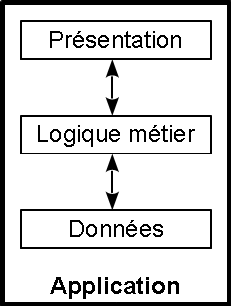
\includegraphics[width=2cm]{img/architecture_3_tiers.png}
%	\caption{Architecture 3 tiers}
%	\label{architecture_3_tiers}
%\end{figure}
~~\\

Le groupe Limagrain travaille dans un environnement Micosoft et utilise ainsi leurs technologies et logiciels, comme par exemple : Windows pour le système d'exploitation, Internet Explorer comme navigateur internet, Outlook comme messagerie, \ldots

Pour développer cette solution nous nous sommes donc tourné vers les technologies Microsoft, facilitant ainsi la compatibilité et l'intégration des composants.

%%%%%%%%%%%%%%%%%%%%%%%%%%%%%%%%%%%%%%%%%%%%%%%%%%%%%%%%%%%%%%%%%%%%%%%%%%%
%%%%%%%%%%%%%%%%%%%%%%%%%%%%%%%%%%%%%%%%%%%%%%%%%%%%%%%%%%%%%%%%%%%%%%%%%%%
%%%%%%%%%%%%%%%%%%%%%%%%%%%%%%%%%%%%%%%%%%%%%%%%%%%%%%%%%%%%%%%%%%%%%%%%%%%

\subsection{Socle}

% TODO: socle = framework ?
La solution développée se base sur un socle existant, développé dans le cadre d'un autre projet. Ceci nous a permis un gain de temps important car une partie importante du projet n'a du être développé à nouveau. En contre partie, les différentes technologies utilisées, qui seront présentées dans cette partie, nous ont été imposées.

%%%%%%%%%%%%%%%%%%%%%%%%%%%%%%%%%%%%%%%%%%%%%%%%%%%%%%%%%%%%%%%%%%%%%%%%%%%

\subsubsection{Gestion des utilisateurs}

Le socle permet une gestion des utilisateurs de l'application. Il est possible de les créer, modifier ou supprimer, pour restreindre l'accès aux personnes autorisées. De plus, il est possible de connecter l'application à un LDAP.
\\

Le \textit{LDAP}, pour Lightweight Directory Access Protocol, est un protocole standard de gestion d'utilisateurs. Son objectif est de centraliser les informations des utilisateurs (nom, identifiant, mot de passe, \ldots) dans un annuaire.

Le principal avantage de cette solution est la mise en commun des comptes utilisateurs, ce qui permet l'utilisateur d'un seul et même compte pour tous les services connectés : Windows, la boite mail Outlook, cette application, \ldots. La figure \ref{LDAP} représente l'interaction des applications avec un LDAP.
%\begin{figure}[!h]
%	\center
%	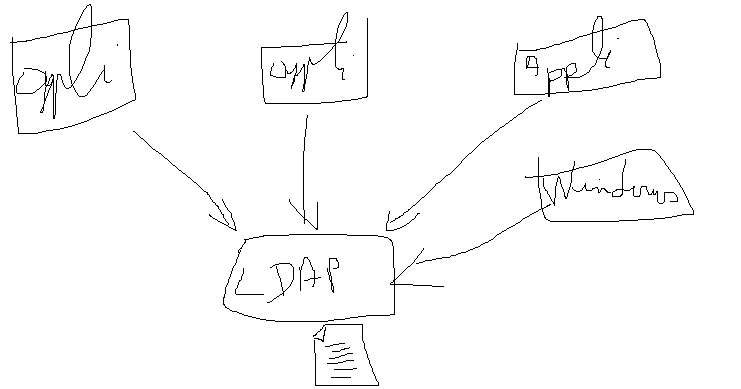
\includegraphics[width=2cm]{img/LDAP.png}
%	\caption{Schéma d'un LDAP}
%	\label{LDAP}
%\end{figure}

%%%%%%%%%%%%%%%%%%%%%%%%%%%%%%%%%%%%%%%%%%%%%%%%%%%%%%%%%%%%%%%%%%%%%%%%%%%

\subsubsection{Gestion des droits}

Il est aussi possible de gérer des droits dans l'application grâce à ce socle. L'objectif est de contrôler les accès et les actions aux utilisateurs ayant le droit, pour protéger les informations confidentielles.
\\

Chaque écran de l'application peut avoir leur accès ou certaines actions restreintes en fonction d'un \textit{droit}. Ceux-ci peuvent prendre trois valeur : 
\begin{itemize}
	\item "aucun accès", par défaut, qui interdit tout accès à l'écran ;
	\item "lecture" n'autorise que l'accès à l'écran, avec la possibilité d'effectuer des recherches ou d'afficher les détails ;
	\item "lecture et écriture" autorise toutes les actions possibles.
\end{itemize}

Un \textit{profil} est un ensemble de droits, qui permet de définir un périmètre d'action. Par exemple un profil "administrateur" aura tous les droits dans l'application, un profil "manager" n'aura que des droits de lecture, ou encore un profil "ressource humaine" possèdera les droits liés aux candidats et contrats, \ldots

Chaque utilisateur possède un ou plusieurs profils, ce qui permet de définir l'ensemble de ses droits. L'utilisation de profils plutôt que de directement de droit permet un gain de temps, car la personne administrant les utilisateurs n'aura pas à affecter les nombreux droits aux nouveaux utilisateurs, et la modification d'un profil permet d'impacter l'ensemble des utilisateurs associés.
\\

La figure \ref{utilisateur_profils_droits} représente le schéma UML des utilisateurs, profils et droits dans l'application.
%\begin{figure}[!h]
%	\center
%	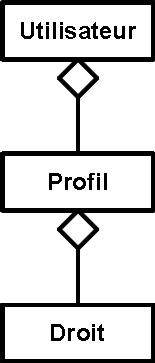
\includegraphics[width=2cm]{img/utilisateur_profils_droits.png}
%	\caption{Utilisation des profils et droits des utilisateurs}
%	\label{utilisateur_profils_droits}
%\end{figure}

%%%%%%%%%%%%%%%%%%%%%%%%%%%%%%%%%%%%%%%%%%%%%%%%%%%%%%%%%%%%%%%%%%%%%%%%%%%
%%%%%%%%%%%%%%%%%%%%%%%%%%%%%%%%%%%%%%%%%%%%%%%%%%%%%%%%%%%%%%%%%%%%%%%%%%%
%%%%%%%%%%%%%%%%%%%%%%%%%%%%%%%%%%%%%%%%%%%%%%%%%%%%%%%%%%%%%%%%%%%%%%%%%%%

\subsection{Langage de programmation}

%%%%%%%%%%%%%%%%%%%%%%%%%%%%%%%%%%%%%%%%%%%%%%%%%%%%%%%%%%%%%%%%%%%%%%%%%%%

\subsubsection{Microsoft .NET Framework}

\textit{.NET Framework} est une plateforme application proposée par Microsoft. Cette technologie est comparable et directement concurrente de Java d'Oracle.

Ce framework est constitués de nombreux composants, disposés en couches au fur et à mesure de ses versions, schématisés sur la figure \ref{.NET_Framework} :
\begin{enumerate}
	\item Le moteur d'exécution appelé Common Language Runtime (CLR) permet de compiler le code course en un langage intermédiaire appelé Microsoft Intermediate Language (MSIL). Ce code est ensuite compilé à la volée lors de la première exécution grâce au compilateur "Just In Time" (JIT) ;
	\item Une bibliothèque de classes, offrant des fonctionnalités de base pour les différentes applications ;
	\item Plusieurs couches supplémentaires proposant des outils de développement d'interfaces graphique (WinForms), d'accès aux données (ADO.NET (Entity Framework)), \ldots
%	\item Une couche de trois composants : WinForms (ou Windows Forms) pour le développement d'interfaces graphiques, ASP.NET permettant la création de sites web dynamiques, et ADO.NET pour l'accès aux bases de données ;
%	\item La version 3.0 apporte Windows Presentation Foundation (WPF) permettant le développement d'applications graphiques vectorielles basées sur le XML, Windows Communication Foundation (WCF) pour la communication, Windows Workflow Foundation (WF) une technologie de gestion des workflow, et enfin Windows CardSpace pour la gestion d'identités ;
\end{enumerate}

%%%%%%%%%%%%%%%%%%%%%%%%%%%%%%%%%%%%%%%%%%%%%%%%%%%%%%%%%%%%%%%%%%%%%%%%%%%

\subsubsection{VB.NET}

\textit{Visual Basic .NET} est un langage de programmation développé par Microsoft. Il s'agit d'une évolution majeure de Visual Basic 6, introduisant l'aspect orienté objet. De plus, le code est compilé dans un langage intermédiaire, appelé Common Intermediate Language (CIL), au même titre que les autres langages fonctionnant sur la machine virtuelle .Net. Ce langage est très proche du C\#, à la syntaxe près.

Le projet a été développé dans ce langage, aussi bien la couche métier que dans la couche présentation.

%%%%%%%%%%%%%%%%%%%%%%%%%%%%%%%%%%%%%%%%%%%%%%%%%%%%%%%%%%%%%%%%%%%%%%%%%%%
%%%%%%%%%%%%%%%%%%%%%%%%%%%%%%%%%%%%%%%%%%%%%%%%%%%%%%%%%%%%%%%%%%%%%%%%%%%
%%%%%%%%%%%%%%%%%%%%%%%%%%%%%%%%%%%%%%%%%%%%%%%%%%%%%%%%%%%%%%%%%%%%%%%%%%%

\subsection{Base de données}

Une \textit{base de données} permet de stocker un grand nombre d'informations ayant des natures différentes. Ces informations sont stockées dans des tables, où les clés permettent de définir les liens de dépendant entre les informations.

%%%%%%%%%%%%%%%%%%%%%%%%%%%%%%%%%%%%%%%%%%%%%%%%%%%%%%%%%%%%%%%%%%%%%%%%%%%

\subsubsection{SQL Server 2008}

Il existe de nombreux système de gestion de base de données : Oracle, MySQL, PostgreSQL, \ldots Nous avons utilisé \textit{Microsoft SQL Server}, dans sa version 2008 R2, par demande du client.

TODO: licence : ce choix car licence déjà achetée pour d'autres ?

%%%%%%%%%%%%%%%%%%%%%%%%%%%%%%%%%%%%%%%%%%%%%%%%%%%%%%%%%%%%%%%%%%%%%%%%%%%

\subsubsection{Mapping de la base de données}

Le \textit{modèle relationnel} est utilisé dans les systèmes de gestion de base de données (SGBD) pour rassembler un ensemble d'informations. Les données (clés) sont dupliquées entre les tables et l'accès aux relations s'effectue ensuite grâce à des jointures entre les tables.

Le \textit{modèle objet}, quant à lui, est utilisé dans la programmation orientée objet. Les données sont modélisées sous la formes d'objets, entités complexes ayant des comportements et des relations entre elles.
\\

Le \textit{mapping objet-relationnel} consiste à interfacer le modèle relationnel d'une base de données avec le modèle orienté objet d'un programme informatique. Généralement, une classe modélisera une table, et attribut d'objet modélisera un champ d'une table, avec un type similaire (par exemple \lstinline{String} pour \lstinline{varchar}).
\\

Cette opération peut être faite à l'aide d'un framework (TODO: glossaire), permettent de s'abstraire de la base de données, automatisant et réduisant ainsi la duplication de code. L'objectif est de faciliter le développement, augmenter la maintenabilité du programme, ou encore s'abstenir du type de base de données.

Microsoft propose plusieurs framework, et c'est \textit{Entity Framework} qui a été utilisé. Il est intégré à Visual Studio, ce qui permet une génération et un paramétrage facilité. De plus, il permet l'interaction avec  LINQ (Language-Integrated Query), extension du langage permettant de faire des requêtes sur des ensembles de données s'abstrayant du type.

%%%%%%%%%%%%%%%%%%%%%%%%%%%%%%%%%%%%%%%%%%%%%%%%%%%%%%%%%%%%%%%%%%%%%%%%%%%
%%%%%%%%%%%%%%%%%%%%%%%%%%%%%%%%%%%%%%%%%%%%%%%%%%%%%%%%%%%%%%%%%%%%%%%%%%%
%%%%%%%%%%%%%%%%%%%%%%%%%%%%%%%%%%%%%%%%%%%%%%%%%%%%%%%%%%%%%%%%%%%%%%%%%%%

\subsection{Les services}

%%%%%%%%%%%%%%%%%%%%%%%%%%%%%%%%%%%%%%%%%%%%%%%%%%%%%%%%%%%%%%%%%%%%%%%%%%%

\subsubsection{Fonction}

La couche de \textit{service} est la partie métier de l'application. Cela permet de séparer le code source lié à l'affichage destiné à l'utilisateur, du code métier effectuant des manipulations dans la base de données.

%%%%%%%%%%%%%%%%%%%%%%%%%%%%%%%%%%%%%%%%%%%%%%%%%%%%%%%%%%%%%%%%%%%%%%%%%%%

\subsubsection{Client-Serveur}

\Jparagraph{Web service}

Un \textit{service web} (ou \textit{web service}) est un programme informatique permettant la communication et l'échange d'informations entre des systèmes hétérogènes et distribués (local, réseau, internet, \ldots), exposant ainsi des fonctionnalités.

L'échange d'informations entre le client et le serveur se fait par sérialisation, consistant à coder les informations contenues en mémoire. Cela peut se faire sous le format texte (XML, JSON, \ldots) ou au format binaire.


\Jparagraph{Windows Communication Foundation}

\textit{Windows Communication Foundation}, couramment appelé sous ses initiales WCF, est la couche de communication de .NET Framework. Cette technologie respecte les normes standards des services web, ce qui lui permet d'appeler ou d'être appelé par des technologies différentes (Java, Python, \ldots).

(TODO: aucun rapport avec WCF, mais plutôt Silverlight ?)
Les différents appels du service web se font de façon asynchrone : le client n'attend pas la réponse du serveur pour continuer son traitement. Cette solution permet de ne pas bloquer l'interface de l'utilisateur, qui pourrait penser à un plantage de l'application. Mais l'inconvénient est l'augmentation de la complexité de programmation car il est nécessaire de contrôler plusieurs fils d'exécution en parallèle.


\Jparagraph{WCF RIA Services}

Il est souvent nécessaire de posséder une logique applicative à la fois du coté serveur que du coté client. C'est le cas par exemple lorsque l'on souhaite vérifier la validité des données avant de les insérer en base de données : soit on effectue la même vérification du coté client et serveur, ce qui impose de dupliquer le code dans les deux couches, soit on n'effectue la vérification coté serveur, ce qui impose une communication inutile entre client et serveur.

Pour éviter ce problème, Microsoft propose le framework \textit{WCF RIA Services}. Cet outil génère du code, contenu du coté serveur, dans la couche client, lors de la compilation.
\\


La figure \ref{WCF_RIA_Services} représente les échanges entre la partie cliente de l'application et la partie serveur.
%\begin{figure}[!h]
%	\center
%	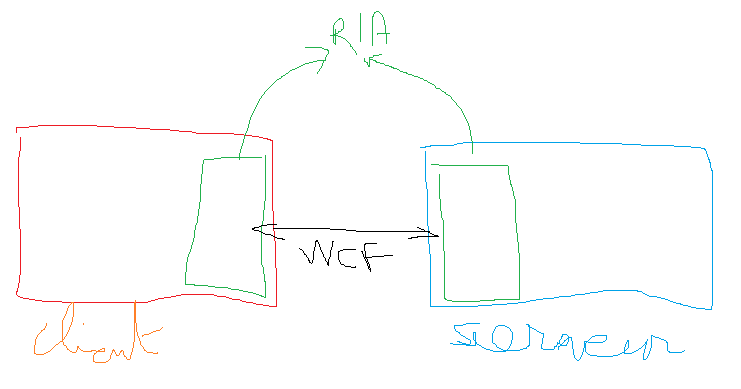
\includegraphics[width=2cm]{img/WCF_RIA_Services.png}
%	\caption{Fonctionnement de l'application client-serveur}
%	\label{WCF_RIA_Services}
%\end{figure}

%%%%%%%%%%%%%%%%%%%%%%%%%%%%%%%%%%%%%%%%%%%%%%%%%%%%%%%%%%%%%%%%%%%%%%%%%%%
%%%%%%%%%%%%%%%%%%%%%%%%%%%%%%%%%%%%%%%%%%%%%%%%%%%%%%%%%%%%%%%%%%%%%%%%%%%
%%%%%%%%%%%%%%%%%%%%%%%%%%%%%%%%%%%%%%%%%%%%%%%%%%%%%%%%%%%%%%%%%%%%%%%%%%%

\subsection{Interface utilisateur}

%%%%%%%%%%%%%%%%%%%%%%%%%%%%%%%%%%%%%%%%%%%%%%%%%%%%%%%%%%%%%%%%%%%%%%%%%%%

\subsubsection{Silverlight}

Microsoft \textit{Silverlight} est un plugin pour navigateur web. Il permet le développement d'applications riches et de pousser plus loin l'expérience utilisateur du web 2.0, au même titre qu'Adobe Flash dont il se veut une alternative. Initialement prévu pour des applications web dans un navigateur, les programmes peuvent être téléchargées pour être utilisés directement sur l'ordinateur ("out of browser"), et permettent aussi le développement d'applications pour Windows Phone 7.

Cette technologie nécessite l'installation du plugin, qui est un sous-ensemble de Microsoft .NET Framework. Les applications sont ainsi cross-browser (Internet Explorer, Firefox, Chrome, \ldots) et cross-platform (Windows, OS-X et Linux, via le projet open-source Moonlight). De plus les applications fonctionnent dans une "sandbox" ("bac a sable") ce qui permet de garantir une sécurité accrue pour l'utilisateur et le serveur.







-----------------------------------------








%%%%%%%%%% Chapitre 3 %%%%%%%%%%
\chapter{Chapter 3}

\section{Section 3.1}

\subsection{SubSection 3.1.1}

\subsubsection{SubSubSection 3.1.1.1}

bla bla bla bla bla bla bla bla bla bla bla bla bla bla bla bla bla bla bla bla bla bla bla bla bla bla bla bla bla bla bla bla bla bla bla bla bla bla bla bla bla bla bla bla bla bla bla bla bla bla bla bla bla bla bla bla bla bla bla bla bla bla bla bla bla bla bla bla bla bla bla bla bla bla bla bla bla bla bla bla bla bla bla bla bla bla bla bla bla bla bla bla.

bla bla bla bla bla bla bla bla bla bla bla bla bla bla bla bla bla bla bla bla bla bla bla bla bla bla bla bla bla bla bla bla bla bla bla bla bla bla bla bla bla bla bla bla bla bla bla bla bla bla bla bla bla bla bla bla bla bla bla bla bla bla bla bla bla bla bla bla bla bla bla bla bla bla bla bla bla bla bla bla bla bla bla bla bla bla bla bla bla bla bla bla.
\\


bla bla bla bla bla bla bla bla bla bla bla bla bla bla bla bla bla bla bla bla bla bla bla bla bla bla bla bla bla bla bla bla bla bla bla bla bla bla bla bla bla bla bla bla bla bla bla bla bla bla bla bla bla bla bla bla bla bla bla bla bla bla bla bla bla bla bla bla bla bla bla bla bla bla bla bla bla bla bla bla bla bla bla bla bla bla bla bla bla bla bla bla.

bla bla bla bla bla bla bla bla bla bla bla bla bla bla bla bla bla bla bla bla bla bla bla bla bla bla bla bla bla bla bla bla bla bla bla bla bla bla bla bla bla bla bla bla bla bla bla bla bla bla bla bla bla bla bla bla bla bla bla bla bla bla bla bla bla bla bla bla bla bla bla bla bla bla bla bla bla bla bla bla bla bla bla bla bla bla bla bla bla bla bla bla.
\\


\subsubsection{SubSubSection 3.1.1.2}

bla bla bla bla bla bla bla bla bla bla bla bla bla bla bla bla bla bla bla bla bla bla bla bla bla bla bla bla bla bla bla bla bla bla bla bla bla bla bla bla bla bla bla bla bla bla bla bla bla bla bla bla bla bla bla bla bla bla bla bla bla bla bla bla bla bla bla bla bla bla bla bla bla bla bla bla bla bla bla bla bla bla bla bla bla bla bla bla bla bla bla bla.

bla bla bla bla bla bla bla bla bla bla bla bla bla bla bla bla bla bla bla bla bla bla bla bla bla bla bla bla bla bla bla bla bla bla bla bla bla bla bla bla bla bla bla bla bla bla bla bla bla bla bla bla bla bla bla bla bla bla bla bla bla bla bla bla bla bla bla bla bla bla bla bla bla bla bla bla bla bla bla bla bla bla bla bla bla bla bla bla bla bla bla bla.
\\


bla bla bla bla bla bla bla bla bla bla bla bla bla bla bla bla bla bla bla bla bla bla bla bla bla bla bla bla bla bla bla bla bla bla bla bla bla bla bla bla bla bla bla bla bla bla bla bla bla bla bla bla bla bla bla bla bla bla bla bla bla bla bla bla bla bla bla bla bla bla bla bla bla bla bla bla bla bla bla bla bla bla bla bla bla bla bla bla bla bla bla bla.

bla bla bla bla bla bla bla bla bla bla bla bla bla bla bla bla bla bla bla bla bla bla bla bla bla bla bla bla bla bla bla bla bla bla bla bla bla bla bla bla bla bla bla bla bla bla bla bla bla bla bla bla bla bla bla bla bla bla bla bla bla bla bla bla bla bla bla bla bla bla bla bla bla bla bla bla bla bla bla bla bla bla bla bla bla bla bla bla bla bla bla bla.
\\


\subsection{SubSection 3.1.2}

\subsubsection{SubSubSection 3.1.2.1}

bla bla bla bla bla bla bla bla bla bla bla bla bla bla bla bla bla bla bla bla bla bla bla bla bla bla bla bla bla bla bla bla bla bla bla bla bla bla bla bla bla bla bla bla bla bla bla bla bla bla bla bla bla bla bla bla bla bla bla bla bla bla bla bla bla bla bla bla bla bla bla bla bla bla bla bla bla bla bla bla bla bla bla bla bla bla bla bla bla bla bla bla.

bla bla bla bla bla bla bla bla bla bla bla bla bla bla bla bla bla bla bla bla bla bla bla bla bla bla bla bla bla bla bla bla bla bla bla bla bla bla bla bla bla bla bla bla bla bla bla bla bla bla bla bla bla bla bla bla bla bla bla bla bla bla bla bla bla bla bla bla bla bla bla bla bla bla bla bla bla bla bla bla bla bla bla bla bla bla bla bla bla bla bla bla.
\\


bla bla bla bla bla bla bla bla bla bla bla bla bla bla bla bla bla bla bla bla bla bla bla bla bla bla bla bla bla bla bla bla bla bla bla bla bla bla bla bla bla bla bla bla bla bla bla bla bla bla bla bla bla bla bla bla bla bla bla bla bla bla bla bla bla bla bla bla bla bla bla bla bla bla bla bla bla bla bla bla bla bla bla bla bla bla bla bla bla bla bla bla.

bla bla bla bla bla bla bla bla bla bla bla bla bla bla bla bla bla bla bla bla bla bla bla bla bla bla bla bla bla bla bla bla bla bla bla bla bla bla bla bla bla bla bla bla bla bla bla bla bla bla bla bla bla bla bla bla bla bla bla bla bla bla bla bla bla bla bla bla bla bla bla bla bla bla bla bla bla bla bla bla bla bla bla bla bla bla bla bla bla bla bla bla.
\\


\subsubsection{SubSubSection 3.1.2.2}

bla bla bla bla bla bla bla bla bla bla bla bla bla bla bla bla bla bla bla bla bla bla bla bla bla bla bla bla bla bla bla bla bla bla bla bla bla bla bla bla bla bla bla bla bla bla bla bla bla bla bla bla bla bla bla bla bla bla bla bla bla bla bla bla bla bla bla bla bla bla bla bla bla bla bla bla bla bla bla bla bla bla bla bla bla bla bla bla bla bla bla bla.

bla bla bla bla bla bla bla bla bla bla bla bla bla bla bla bla bla bla bla bla bla bla bla bla bla bla bla bla bla bla bla bla bla bla bla bla bla bla bla bla bla bla bla bla bla bla bla bla bla bla bla bla bla bla bla bla bla bla bla bla bla bla bla bla bla bla bla bla bla bla bla bla bla bla bla bla bla bla bla bla bla bla bla bla bla bla bla bla bla bla bla bla.
\\


bla bla bla bla bla bla bla bla bla bla bla bla bla bla bla bla bla bla bla bla bla bla bla bla bla bla bla bla bla bla bla bla bla bla bla bla bla bla bla bla bla bla bla bla bla bla bla bla bla bla bla bla bla bla bla bla bla bla bla bla bla bla bla bla bla bla bla bla bla bla bla bla bla bla bla bla bla bla bla bla bla bla bla bla bla bla bla bla bla bla bla bla.

bla bla bla bla bla bla bla bla bla bla bla bla bla bla bla bla bla bla bla bla bla bla bla bla bla bla bla bla bla bla bla bla bla bla bla bla bla bla bla bla bla bla bla bla bla bla bla bla bla bla bla bla bla bla bla bla bla bla bla bla bla bla bla bla bla bla bla bla bla bla bla bla bla bla bla bla bla bla bla bla bla bla bla bla bla bla bla bla bla bla bla bla.
\\


\section{Section 3.2}

\subsection{SubSection 3.2.1}

\subsubsection{SubSubSection 3.2.1.1}

bla bla bla bla bla bla bla bla bla bla bla bla bla bla bla bla bla bla bla bla bla bla bla bla bla bla bla bla bla bla bla bla bla bla bla bla bla bla bla bla bla bla bla bla bla bla bla bla bla bla bla bla bla bla bla bla bla bla bla bla bla bla bla bla bla bla bla bla bla bla bla bla bla bla bla bla bla bla bla bla bla bla bla bla bla bla bla bla bla bla bla bla.

bla bla bla bla bla bla bla bla bla bla bla bla bla bla bla bla bla bla bla bla bla bla bla bla bla bla bla bla bla bla bla bla bla bla bla bla bla bla bla bla bla bla bla bla bla bla bla bla bla bla bla bla bla bla bla bla bla bla bla bla bla bla bla bla bla bla bla bla bla bla bla bla bla bla bla bla bla bla bla bla bla bla bla bla bla bla bla bla bla bla bla bla.
\\


bla bla bla bla bla bla bla bla bla bla bla bla bla bla bla bla bla bla bla bla bla bla bla bla bla bla bla bla bla bla bla bla bla bla bla bla bla bla bla bla bla bla bla bla bla bla bla bla bla bla bla bla bla bla bla bla bla bla bla bla bla bla bla bla bla bla bla bla bla bla bla bla bla bla bla bla bla bla bla bla bla bla bla bla bla bla bla bla bla bla bla bla.

bla bla bla bla bla bla bla bla bla bla bla bla bla bla bla bla bla bla bla bla bla bla bla bla bla bla bla bla bla bla bla bla bla bla bla bla bla bla bla bla bla bla bla bla bla bla bla bla bla bla bla bla bla bla bla bla bla bla bla bla bla bla bla bla bla bla bla bla bla bla bla bla bla bla bla bla bla bla bla bla bla bla bla bla bla bla bla bla bla bla bla bla.
\\


\subsubsection{SubSubSection 3.2.1.2}

bla bla bla bla bla bla bla bla bla bla bla bla bla bla bla bla bla bla bla bla bla bla bla bla bla bla bla bla bla bla bla bla bla bla bla bla bla bla bla bla bla bla bla bla bla bla bla bla bla bla bla bla bla bla bla bla bla bla bla bla bla bla bla bla bla bla bla bla bla bla bla bla bla bla bla bla bla bla bla bla bla bla bla bla bla bla bla bla bla bla bla bla.

bla bla bla bla bla bla bla bla bla bla bla bla bla bla bla bla bla bla bla bla bla bla bla bla bla bla bla bla bla bla bla bla bla bla bla bla bla bla bla bla bla bla bla bla bla bla bla bla bla bla bla bla bla bla bla bla bla bla bla bla bla bla bla bla bla bla bla bla bla bla bla bla bla bla bla bla bla bla bla bla bla bla bla bla bla bla bla bla bla bla bla bla.
\\


bla bla bla bla bla bla bla bla bla bla bla bla bla bla bla bla bla bla bla bla bla bla bla bla bla bla bla bla bla bla bla bla bla bla bla bla bla bla bla bla bla bla bla bla bla bla bla bla bla bla bla bla bla bla bla bla bla bla bla bla bla bla bla bla bla bla bla bla bla bla bla bla bla bla bla bla bla bla bla bla bla bla bla bla bla bla bla bla bla bla bla bla.

bla bla bla bla bla bla bla bla bla bla bla bla bla bla bla bla bla bla bla bla bla bla bla bla bla bla bla bla bla bla bla bla bla bla bla bla bla bla bla bla bla bla bla bla bla bla bla bla bla bla bla bla bla bla bla bla bla bla bla bla bla bla bla bla bla bla bla bla bla bla bla bla bla bla bla bla bla bla bla bla bla bla bla bla bla bla bla bla bla bla bla bla.
\\


\subsection{SubSection 3.2.2}

\subsubsection{SubSubSection 3.2.2.1}

bla bla bla bla bla bla bla bla bla bla bla bla bla bla bla bla bla bla bla bla bla bla bla bla bla bla bla bla bla bla bla bla bla bla bla bla bla bla bla bla bla bla bla bla bla bla bla bla bla bla bla bla bla bla bla bla bla bla bla bla bla bla bla bla bla bla bla bla bla bla bla bla bla bla bla bla bla bla bla bla bla bla bla bla bla bla bla bla bla bla bla bla.

bla bla bla bla bla bla bla bla bla bla bla bla bla bla bla bla bla bla bla bla bla bla bla bla bla bla bla bla bla bla bla bla bla bla bla bla bla bla bla bla bla bla bla bla bla bla bla bla bla bla bla bla bla bla bla bla bla bla bla bla bla bla bla bla bla bla bla bla bla bla bla bla bla bla bla bla bla bla bla bla bla bla bla bla bla bla bla bla bla bla bla bla.
\\


bla bla bla bla bla bla bla bla bla bla bla bla bla bla bla bla bla bla bla bla bla bla bla bla bla bla bla bla bla bla bla bla bla bla bla bla bla bla bla bla bla bla bla bla bla bla bla bla bla bla bla bla bla bla bla bla bla bla bla bla bla bla bla bla bla bla bla bla bla bla bla bla bla bla bla bla bla bla bla bla bla bla bla bla bla bla bla bla bla bla bla bla.

bla bla bla bla bla bla bla bla bla bla bla bla bla bla bla bla bla bla bla bla bla bla bla bla bla bla bla bla bla bla bla bla bla bla bla bla bla bla bla bla bla bla bla bla bla bla bla bla bla bla bla bla bla bla bla bla bla bla bla bla bla bla bla bla bla bla bla bla bla bla bla bla bla bla bla bla bla bla bla bla bla bla bla bla bla bla bla bla bla bla bla bla.
\\


\subsubsection{SubSubSection 3.2.2.2}

bla bla bla bla bla bla bla bla bla bla bla bla bla bla bla bla bla bla bla bla bla bla bla bla bla bla bla bla bla bla bla bla bla bla bla bla bla bla bla bla bla bla bla bla bla bla bla bla bla bla bla bla bla bla bla bla bla bla bla bla bla bla bla bla bla bla bla bla bla bla bla bla bla bla bla bla bla bla bla bla bla bla bla bla bla bla bla bla bla bla bla bla.

bla bla bla bla bla bla bla bla bla bla bla bla bla bla bla bla bla bla bla bla bla bla bla bla bla bla bla bla bla bla bla bla bla bla bla bla bla bla bla bla bla bla bla bla bla bla bla bla bla bla bla bla bla bla bla bla bla bla bla bla bla bla bla bla bla bla bla bla bla bla bla bla bla bla bla bla bla bla bla bla bla bla bla bla bla bla bla bla bla bla bla bla.
\\


bla bla bla bla bla bla bla bla bla bla bla bla bla bla bla bla bla bla bla bla bla bla bla bla bla bla bla bla bla bla bla bla bla bla bla bla bla bla bla bla bla bla bla bla bla bla bla bla bla bla bla bla bla bla bla bla bla bla bla bla bla bla bla bla bla bla bla bla bla bla bla bla bla bla bla bla bla bla bla bla bla bla bla bla bla bla bla bla bla bla bla bla.

bla bla bla bla bla bla bla bla bla bla bla bla bla bla bla bla bla bla bla bla bla bla bla bla bla bla bla bla bla bla bla bla bla bla bla bla bla bla bla bla bla bla bla bla bla bla bla bla bla bla bla bla bla bla bla bla bla bla bla bla bla bla bla bla bla bla bla bla bla bla bla bla bla bla bla bla bla bla bla bla bla bla bla bla bla bla bla bla bla bla bla bla.
\\


%%%%%%%%%% Conclusion %%%%%%%%%%
\cleardoublepage

\chapter*{Conclusion}

\addcontentsline{toc}{chapter}{Conclusion}
\markboth{Conclusion}{}



% Rapppel du sujet
Intégré à une société de services en ingénierie informatique, j'ai participé à l'élaboration de trois projets distincts.
\\

% Etude terminée ?

% Améliorations possibles

% Difficultés rencontrées
Les principaux problèmes rencontrés concernaient la découverte des différentes technologies utilisées, mais aussi les aspects fonctionnels comme la communication avec le client ou la compréhension du besoin.

% Ce que ça m'a apporté
Ce stage m'a permis de découvrir de nouvelles facettes du métier d'ingénieur que je n'ai pas abordé lors de mon stage de seconde année.
Il a permis d'améliorer mes compétences fonctionnelles avec la communication et la compréhension du besoin, mais aussi techniques avec la découverte de nouvelles technologies.

\clearpage
\pagestyle{empty}

%%%%%%%%%% Bibliographie %%%%%%%%%%
\cleardoublepage

\chapter*{Bibliographie}

\addcontentsline{toc}{chapter}{Bibliographie}
\markboth{Bibliographie}{}



bla bla bla bla bla bla bla bla bla bla bla bla bla bla bla bla bla bla bla bla bla bla bla bla bla bla bla bla bla bla bla bla bla bla bla bla bla bla bla bla bla bla bla bla bla bla bla bla bla bla bla bla bla bla bla bla bla bla bla bla bla bla bla bla bla bla bla bla bla bla bla bla bla bla bla bla bla bla bla bla bla bla bla bla bla bla bla bla bla bla bla bla.

bla bla bla bla bla bla bla bla bla bla bla bla bla bla bla bla bla bla bla bla bla bla bla bla bla bla bla bla bla bla bla bla bla bla bla bla bla bla bla bla bla bla bla bla bla bla bla bla bla bla bla bla bla bla bla bla bla bla bla bla bla bla bla bla bla bla bla bla bla bla bla bla bla bla bla bla bla bla bla bla bla bla bla bla bla bla bla bla bla bla bla bla.
\\


bla bla bla bla bla bla bla bla bla bla bla bla bla bla bla bla bla bla bla bla bla bla bla bla bla bla bla bla bla bla bla bla bla bla bla bla bla bla bla bla bla bla bla bla bla bla bla bla bla bla bla bla bla bla bla bla bla bla bla bla bla bla bla bla bla bla bla bla bla bla bla bla bla bla bla bla bla bla bla bla bla bla bla bla bla bla bla bla bla bla bla bla.

bla bla bla bla bla bla bla bla bla bla bla bla bla bla bla bla bla bla bla bla bla bla bla bla bla bla bla bla bla bla bla bla bla bla bla bla bla bla bla bla bla bla bla bla bla bla bla bla bla bla bla bla bla bla bla bla bla bla bla bla bla bla bla bla bla bla bla bla bla bla bla bla bla bla bla bla bla bla bla bla bla bla bla bla bla bla bla bla bla bla bla bla.
\\


bla bla bla bla bla bla bla bla bla bla bla bla bla bla bla bla bla bla bla bla bla bla bla bla bla bla bla bla bla bla bla bla bla bla bla bla bla bla bla bla bla bla bla bla bla bla bla bla bla bla bla bla bla bla bla bla bla bla bla bla bla bla bla bla bla bla bla bla bla bla bla bla bla bla bla bla bla bla bla bla bla bla bla bla bla bla bla bla bla bla bla bla.

bla bla bla bla bla bla bla bla bla bla bla bla bla bla bla bla bla bla bla bla bla bla bla bla bla bla bla bla bla bla bla bla bla bla bla bla bla bla bla bla bla bla bla bla bla bla bla bla bla bla bla bla bla bla bla bla bla bla bla bla bla bla bla bla bla bla bla bla bla bla bla bla bla bla bla bla bla bla bla bla bla bla bla bla bla bla bla bla bla bla bla bla.
\\


bla bla bla bla bla bla bla bla bla bla bla bla bla bla bla bla bla bla bla bla bla bla bla bla bla bla bla bla bla bla bla bla bla bla bla bla bla bla bla bla bla bla bla bla bla bla bla bla bla bla bla bla bla bla bla bla bla bla bla bla bla bla bla bla bla bla bla bla bla bla bla bla bla bla bla bla bla bla bla bla bla bla bla bla bla bla bla bla bla bla bla bla.

bla bla bla bla bla bla bla bla bla bla bla bla bla bla bla bla bla bla bla bla bla bla bla bla bla bla bla bla bla bla bla bla bla bla bla bla bla bla bla bla bla bla bla bla bla bla bla bla bla bla bla bla bla bla bla bla bla bla bla bla bla bla bla bla bla bla bla bla bla bla bla bla bla bla bla bla bla bla bla bla bla bla bla bla bla bla bla bla bla bla bla bla.
\\


bla bla bla bla bla bla bla bla bla bla bla bla bla bla bla bla bla bla bla bla bla bla bla bla bla bla bla bla bla bla bla bla bla bla bla bla bla bla bla bla bla bla bla bla bla bla bla bla bla bla bla bla bla bla bla bla bla bla bla bla bla bla bla bla bla bla bla bla bla bla bla bla bla bla bla bla bla bla bla bla bla bla bla bla bla bla bla bla bla bla bla bla.

bla bla bla bla bla bla bla bla bla bla bla bla bla bla bla bla bla bla bla bla bla bla bla bla bla bla bla bla bla bla bla bla bla bla bla bla bla bla bla bla bla bla bla bla bla bla bla bla bla bla bla bla bla bla bla bla bla bla bla bla bla bla bla bla bla bla bla bla bla bla bla bla bla bla bla bla bla bla bla bla bla bla bla bla bla bla bla bla bla bla bla bla.
\\


bla bla bla bla bla bla bla bla bla bla bla bla bla bla bla bla bla bla bla bla bla bla bla bla bla bla bla bla bla bla bla bla bla bla bla bla bla bla bla bla bla bla bla bla bla bla bla bla bla bla bla bla bla bla bla bla bla bla bla bla bla bla bla bla bla bla bla bla bla bla bla bla bla bla bla bla bla bla bla bla bla bla bla bla bla bla bla bla bla bla bla bla.

bla bla bla bla bla bla bla bla bla bla bla bla bla bla bla bla bla bla bla bla bla bla bla bla bla bla bla bla bla bla bla bla bla bla bla bla bla bla bla bla bla bla bla bla bla bla bla bla bla bla bla bla bla bla bla bla bla bla bla bla bla bla bla bla bla bla bla bla bla bla bla bla bla bla bla bla bla bla bla bla bla bla bla bla bla bla bla bla bla bla bla bla.
\\


bla bla bla bla bla bla bla bla bla bla bla bla bla bla bla bla bla bla bla bla bla bla bla bla bla bla bla bla bla bla bla bla bla bla bla bla bla bla bla bla bla bla bla bla bla bla bla bla bla bla bla bla bla bla bla bla bla bla bla bla bla bla bla bla bla bla bla bla bla bla bla bla bla bla bla bla bla bla bla bla bla bla bla bla bla bla bla bla bla bla bla bla.

bla bla bla bla bla bla bla bla bla bla bla bla bla bla bla bla bla bla bla bla bla bla bla bla bla bla bla bla bla bla bla bla bla bla bla bla bla bla bla bla bla bla bla bla bla bla bla bla bla bla bla bla bla bla bla bla bla bla bla bla bla bla bla bla bla bla bla bla bla bla bla bla bla bla bla bla bla bla bla bla bla bla bla bla bla bla bla bla bla bla bla bla.
\\


bla bla bla bla bla bla bla bla bla bla bla bla bla bla bla bla bla bla bla bla bla bla bla bla bla bla bla bla bla bla bla bla bla bla bla bla bla bla bla bla bla bla bla bla bla bla bla bla bla bla bla bla bla bla bla bla bla bla bla bla bla bla bla bla bla bla bla bla bla bla bla bla bla bla bla bla bla bla bla bla bla bla bla bla bla bla bla bla bla bla bla bla.

bla bla bla bla bla bla bla bla bla bla bla bla bla bla bla bla bla bla bla bla bla bla bla bla bla bla bla bla bla bla bla bla bla bla bla bla bla bla bla bla bla bla bla bla bla bla bla bla bla bla bla bla bla bla bla bla bla bla bla bla bla bla bla bla bla bla bla bla bla bla bla bla bla bla bla bla bla bla bla bla bla bla bla bla bla bla bla bla bla bla bla bla.
\\


bla bla bla bla bla bla bla bla bla bla bla bla bla bla bla bla bla bla bla bla bla bla bla bla bla bla bla bla bla bla bla bla bla bla bla bla bla bla bla bla bla bla bla bla bla bla bla bla bla bla bla bla bla bla bla bla bla bla bla bla bla bla bla bla bla bla bla bla bla bla bla bla bla bla bla bla bla bla bla bla bla bla bla bla bla bla bla bla bla bla bla bla.

bla bla bla bla bla bla bla bla bla bla bla bla bla bla bla bla bla bla bla bla bla bla bla bla bla bla bla bla bla bla bla bla bla bla bla bla bla bla bla bla bla bla bla bla bla bla bla bla bla bla bla bla bla bla bla bla bla bla bla bla bla bla bla bla bla bla bla bla bla bla bla bla bla bla bla bla bla bla bla bla bla bla bla bla bla bla bla bla bla bla bla bla.

\clearpage
\thispagestyle{empty}

\end{document}